    % !TEX TS-program = pdflatex
\documentclass[tikz,border=10pt]{standalone}
\usepackage{pgfplots}
\pgfplotsset{compat=1.18}
\begin{document}
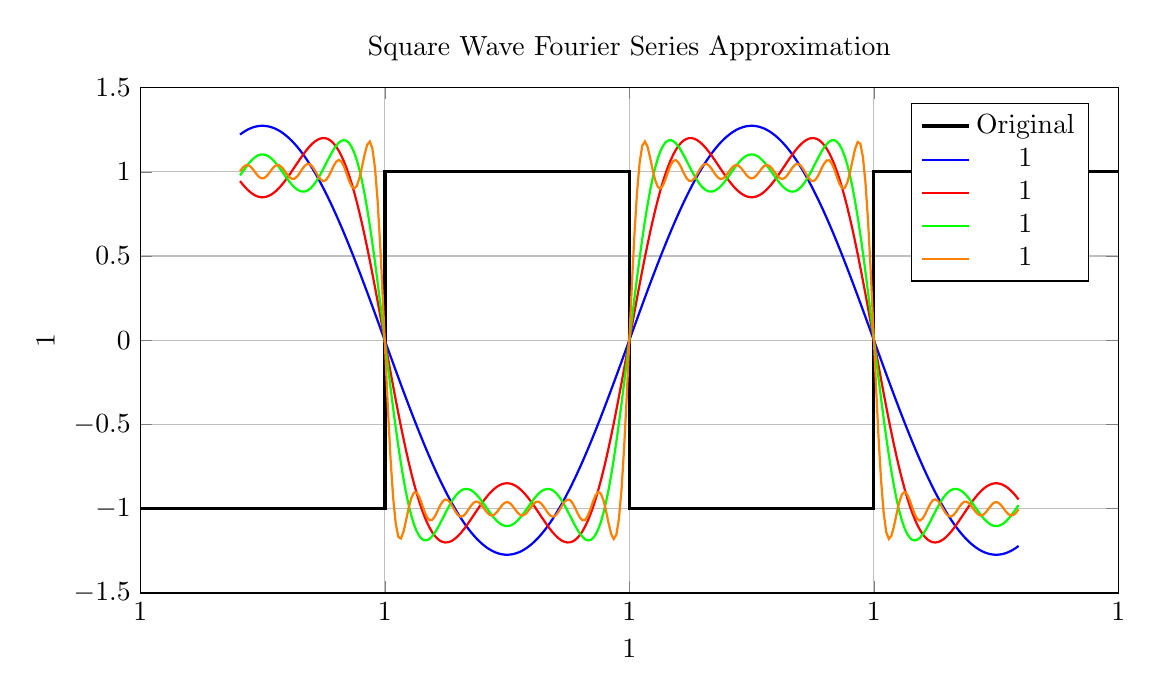
\begin{tikzpicture}
    \begin{axis}[
            width=14cm, height=8cm,
            xlabel={\(1\)},
            ylabel={\(1\)},
            title={Square Wave Fourier Series Approximation},
            xmin=-6.28, xmax=6.28,
            ymin=-1.5, ymax=1.5,
            grid=major,
            legend pos=north east,
            samples=301,
            xtick={-6.28, -3.14, 0, 3.14, 6.28},
            xticklabels={\(1\), \(1\), \(1\), \(1\), \(1\)}
        ]

        % Original square wave
        \addplot[black, very thick, const plot] coordinates {
                (-6.28, -1) (-3.14, -1) (-3.14, 1) (0, 1) (0, -1) (3.14, -1) (3.14, 1) (6.28, 1)
            };
        \addlegendentry{Original}

        % N=1 approximation
        \addplot[blue, thick] {(4/pi)*sin(deg(x))};
        \addlegendentry{\(1\)}

        % N=3 approximation
        \addplot[red, thick] {(4/pi)*(sin(deg(x)) + sin(deg(3*x))/3)};
        \addlegendentry{\(1\)}

        % N=5 approximation
        \addplot[green, thick] {(4/pi)*(sin(deg(x)) + sin(deg(3*x))/3 + sin(deg(5*x))/5)};
        \addlegendentry{\(1\)}

        % N=15 approximation
        \addplot[orange, thick] {(4/pi)*(sin(deg(x)) + sin(deg(3*x))/3 + sin(deg(5*x))/5 + sin(deg(7*x))/7 + sin(deg(9*x))/9 + sin(deg(11*x))/11 + sin(deg(13*x))/13 + sin(deg(15*x))/15)};
        \addlegendentry{\(1\)}

    \end{axis}
\end{tikzpicture}
\end{document}